\documentclass[a4paper,11pt]{report}
% $Revision: 1.16 $
% $Id: SPE780-project-dissertation.tex,v 1.9 2010/06/26 19:25:23
% hendrivi Exp $

\newcommand{\trademark}{\textsuperscript{\texttt{TM}\ }}
\newcommand{\Bad}{BadThing\trademark}
\newcommand{\Good}{GoodThing\trademark}

\usepackage{gcl}
\usepackage{algorithmic}
\usepackage{graphicx}
\usepackage{epstopdf}
\usepackage{natbib}
\usepackage{pfs}
\usepackage{amsmath}
\usepackage{amssymb}
\usepackage{listings}

\usepackage{threeparttable}
\usepackage{colortbl}
\usepackage{xtab}
\usepackage{longtable}

\lstloadlanguages{erlang}
%\lstset{ %
%language=erlang,
%numbers=left,
%numberstyle=\tiny,
%showspaces=false,               % show spaces adding particular underscores
%showstringspaces=false,         % underline spaces within strings
%breaklines=false,                % sets no automatic line breaking
%breakatwhitespace=true        % sets if automatic breaks should only happen at whitespace
%}

\usepackage{algorithmic}
\usepackage{algorithm}

\setlength{\parindent}{15pt}

\newlength{\OBLS}\setlength{\OBLS}{\baselineskip}
\newlength{\OPAR}\setlength{\OPAR}{\parindent}
\newcommand{\pgskip}{\hspace{\mathindent}\=\+}
\newcommand{\FORhv}[1]{\FRM{\,#1\,}}
\newcommand{\FRM}[1]{\mbox{$#1$}}
\newcommand{\DERIVE}
  {\setlength{\baselineskip}{1.3\baselineskip}
  \begin{tabbing}
  \hspace{\OPAR}\=\hspace{\OPAR}\=\hspace{\OPAR}\=\hspace{\OPAR}\=\hspace{\OPAR}\=\hspace{\OPAR}\=\kill
  }
\newcommand{\form}[1]
  {\>\>\FORhv{#1}}
\newcommand{\hint}[2]
  {\\*\>\FRM{#1}\>\>\{#2\}\\}
\newcommand{\STARTPROOF}[1]
  {\TOPROVE{#1}\\$\vartriangleright$ \>\>}
\newcommand{\TOPROVE}[1]
  {#1}
\newcommand{\ENDDERIVE}
  {\end{tabbing}\setlength{\baselineskip}{\OBLS}
}
\newcommand{\ENDPROOF}
  {$\rbrack\arrowvert$\\
  $\square$\\\\}
\newcommand {\IND}
  {\setlength{\parindent}{\OPAR}\\
  \begin{indent}}
\newcommand {\ENDIND}
  {\end{indent}\\
  \setlength{\parindent}{0 pt}\\}
%\newcommand {\IF}
%  {\mathbf{if} \:\:}
\newcommand {\BAR}
  {\ [\!] \:\:\:}
\newcommand {\FI}
  {\mathbf{fi} \:\:}
\newcommand {\ARROW}
  {\rightarrow}
\newcommand{\clearemptydoublepage}{\newpage{\pagestyle{empty}\cleardoublepage}}
\newcommand{\TT} {\textit{true}}
\newcommand{\FF} {\textit{false}}

\usepackage{float}
\newfloat{trace}{tbp}{lop}[section]
\newfloat{tablehv}{tbp}{lop}[section]
\newfloat{Program}{tbp}{lop}[section]
%\floatstyle{plain}
\newfloat{Figure}{htb}{lop}[chapter]
\floatstyle{boxed}
\newfloat{BFigure}{htb}{lop}[chapter]
\floatname{BFigure}{Figure}


\author{Hendrik Visag\`e\\SN:91211108} 
\title{Concurrent Brzozowski
	DFA construction using Erlang
 \\\small{and how it turned out to be a
		Google MapReduce algorithm}}
 \date{\today}

\begin{document}

\lstset{ %
escapeinside={(*@}{@*)},
tabsize=2,
language=erlang,
%basicstyle=\ttfamily,
numbers=left,
identifierstyle=,
keywordstyle=\bfseries,
numberstyle=\tiny,
showtabs=true,
showspaces=true,							 % show spaces adding particular underscores
showstringspaces=true,				 % underline spaces within strings
breaklines=true,%false,								 % sets no automatic line breaking
breakatwhitespace=true				% sets if automatic breaks should only
															% happen at whitespace
}


\maketitle

\chapter{\textit{Raison d'etre}}

\section{Becoming intrigued}

Earlier this year, the author noticed several job advertiments for
Erlang programmers on a South African job advertising
website. Investigating this further, the author became quite intrigued
by the Erlang language claims about concurrency and availability, and
even more so because Erlang is a functional programming language. This
alone is not a good enough reason to learn a language, especially when
there is no task or project per se to code in the language. For that
we need to find a reason to do a task in Erlang. But before we get to
that question problem, let us examine some of the state of some
aspects of Computer Science.

\subsection{Today's CPUs}
Concurrent algorithms are becoming more important lately as the
commodity CPUs shipped on laptops and desktops, are nearly without
exception multi-cored or multithreaded. \cite{ActorModel} already
claimed in 1985 that massive parallelism is the future of computing,
and it obviously have become a trend with CPUs when Intel's
Hyperthreading, Sun's CoolThread
CPUs and multi-core AMD Opteron CPUs got introduced.
The idea is to rather have
more processing units available than to try and raise the core
clockspeeds. This apparently helps to keep CPUs cooler, and provide users more
processing power. However, this necesitates the need for concurrent
algorithms and parallel processing to be able to effectively and
efficiently use the processing power available in these processing
units, as the core clock is not faster, but the number of processing
units increased.
The Oracle\footnote{previously Sun Microsystems} SPARC T3 is at the
extreme end at present with 128 threads across 16cores on a 1.65GHz
CPU
socket.\footnote{http://www.oracle.com/us/products/servers-storage/servers/sparc-enterprise/t-series/sparc-t3-171613.html
accessed 17 October 2010}

\subsection{Determinate Finite Automata (DFA)}
DFAs as a matching algorithm have big importance in the matching of
patterns. These patterns could be virus signatures, DNA or even
network based intrusion detection and prevention. These DFAs are
constructed from regular expressions and as these regular expressions
become more complex and extended, it is but natural to ask how the DFA
construction could be made faster using the available
multi-core and multi-threaded CPUs, and that is the reason for the
research into the concurrency of this algorithm.

We will have to point out that in this research, we focussed on the
construction of the DFA from an expression, and not the actual DFA
application to the data to be matched, nor will this study look into the parsing of the
regular expressions into expressions useful for our DFA construction.


\subsection{Erlang}

Erlang in a functional language and for programmers used to procedural
languages, there is a couple of
interesting features (or some might say annoyances) that would make it
at least a learning experience to guage the language. Armstrong boosts
about Erlang's built-in
concurrency features, and this would be a perfect match to test both
the language on multicore CPUs.

\section{Research focus}



The problem this study addresses, is some research into the concurrency
possibilities of the sequential Brzozowski algorithm and to implement
this in Erlang. This way we will be combining the concurrent features
of todays CPUs, the Erlang language that boasts about its concurrency
features as well as the quest for a concurrent Brzozowski DFA
construction.

\texttt{The rest of this document will first look at Erlang and its feature
set and what makes Erlang (and to some degree functional languages)
different from other programming languages especially its support for
concurrency. Then we will look at the Brzozowski sequential algorithm
and some parallelization proposals.  Lastly we will discuss the Erlang
implementations for the parallelizations proposals.
}
\chapter{Erlang - the language}

\section{Introduction}

In this chapter, we will give some brief overviews to Erlang's history
and it's language constructs. We will also explain those constructs
and ideas that we have used in this project as well as those
constructs that is not obviously the same as in other computer
languages like the C/C++ languages.	 For the purposes of explanation
in later parts, we will briefly give an Erlang language introduction
to some percularities. However, for proper detailed explanations we will refer
the reader to \cite{Armstrong}.



\section{Brief history}

Armstrong \cite{thesis:armstrong} gives a detailed historical overview
of Erlang since it's inception in 1986 till his thesis circa 2001. In
summary it started in 1981 from the goal \emph{``to suggest new
  architectures, concepts and structures for future processing systems
  development''}. Armstrong started to work on adding concurrent
processes to Prolog and the language evolved away from Prolog and
evolved with its own abstract machines (virtual machines in the JAVA
terminology). Erlang have been used in the AXD301 switch which
superceded the failed AXD-N switch and it is claimed to have a
\textbf{NINE} nines\footnote{99.9999999\% where the usual target for
  mission critical systems is 5 nines (99.999\%) while vendors (from
  the authors experiences) do not easily target nor claim uptimes
  higher than 95\%} uptime in production, while still having around
2million lines of Erlang code.

The main theme found in Erlang is to have small parts that shares
nothing while working together, and if any of these small parts
experience problems it can not handle, it rather fail fast and let a
supervisor process handle the failure and to restart the failed
process.

This fail fast is especially nice as there is not suppose to be any
shared memory between processes/parts, which means that a failure in
one process should not impact the other processes by corrupting shared
memory. This is quite a different approach from other threading models
like the C based Posix threads, where process memory (and thus
variables) are shared, and thus have a need for locks and other mutual
exclusion methods to prevent the threads from concurrently accessing
memory, and thereby corrupting data. 

The author would like to point out that this is different from
guaranteed and proven correctness used in software development for
critical software used in aplications like the space shuttles that
can not tolerate any glitches, where as the Erlang model tolerates the
glitches by restarting the processes.

\section{Quick Language Introduction}

In this section, we will briefly introduce the reader to the Erlang
language. This should be sufficient to be able to grasp the code
presented in this research, and  it will not be a detailed
reference. The reader are referred to Armstrong\cite{Armstrong} or
O'Reilly\cite{O'reilly} for further in depth explanations and
references to the Erlang language.

\subsection{atoms and Variables}

Erlang distinguishes between atoms and variables mostly by the first
character being uppercase for variables or a lowercase character for
atoms.\footnote{Yes, there are exceptions but that means quoting
  etc. which have not being used in our code}

Erlang's atoms are similar to C/C++ \texttt{enums}, just more generic
and not typed like the C/C++ enums which are but typed numbers.


\section{Functional language features}

This section we will briefly glance over some of Erlang's
peculiar\footnote{compared to the C and other procedural type
  languages} language features to give the reader a grasp of the
expressive power that helped to produce the programs in such short
time.

\subsection{Pattern Matching - function overloading}
\label{sec:pattern}

One of the strengths of Erlang (and the author understood other
functional languages too, but have not investigated that) is the way
pattern matching is used for code flow paths. Program listing
\ref{prog:pattern} shows this feature with the two functions
\texttt{area/2}, \texttt{area/3} and \texttt{area/4}. Remember the
atoms start with lowercase letters while the Variables that gets bound
to a value, starts with an uppercase letter.

\begin{Program}
\caption{Pattern matching in code flow}
\label{prog:pattern}
\begin{lstlisting}
area(square,Side) -> Side*Side;
area(cube,Side) -> area(square,Side)*6;
area(circle,Radius) -> area(circle,radius,Radius).

area(circle,radius,Radius) -> Radius*Radius*3.14;
area(circle,diameter,Diameter) -> area(circle,radius,Diameter/2);
area(triangle,Base,Height) -> Base*Height/2;
area(rectangle,Height,Width) -> Height*Width.

area(box,Height,Width,Depth) -> ((Height*Width) +
      (Height*Depth) + (Width*Depth))*2.
\end{lstlisting}
\end{Program}

As could be seen in this example, that we used multiple functions (and
have them match based on the parameters) rather than having
if-then-else or case/switch statements to make code flow
decisions. The different distributor states is also handled using
these parameter matching.

\paragraph{Guards} 
\label{par:guards}Another code flow technique is the use of guards
(\texttt{when} statements) inside functions. These help firstly with
pre-conditions (ie. to force only accepting valid values, like
positive values for distance), and secondly with another method of
conrolling the flow of code, but only after the parameters have been
matched (Ie. a parameter could match anything, but we want to handle
the circle and square different).

These same pattern matching and guards is extended to the message
receiving discussed in section \ref{sec:communications} and shown in
program \ref{prog:recexample}

Something else to note here, is that the underscore denotes a
parameter who's value will be unbounded and ignored. Sometimes a
variable with a prepended underscore would be a way to name a
variable that would not be used, to prevent compiler warnings.

\paragraph{Notation of functions}

A convention in the Erlang texts, is to refer to
\textbf{module:function/arity} for a function for example
\texttt{lists:map/2} which is read as
\begin{description}
\item[module] lists
\item[function name] map
\item[arity] taking 2 parameters
\end{description}

\subsection{Functions as first class members}
\label{sec:func1st}
By definition a function in a functional language is a first class
member, where a function can be passed around like a variable. This do
allow for interesting concepts where you have a function definition
inside a function call, for example to map a list to its squares, we
use something like :
%\begin{Program}[H]
\begin{lstlisting}[language=erlang]
lists:map(		fun(X) -> X*X end,
							[1,5,3] )
\end{lstlisting}
%\end{Program}

Here we provide a list with elements \texttt{[1, 5, 3]}, and
\texttt{map/2} take each element of that list, apply the provided
function (in this case \texttt{fun(X) -> X*X}) to that element, and
returns a list with the new values \texttt{[1, 25, 9]}.

\subsection{Imutable variables}
\label{sec:imVar}
Variables in Erlang is like algebraic variables that have a fixed
value during a run of a function block. For example, once you have
bound $X=1$ and then evaluate $Y=X+2$ we will have $Y==3$ and we can
not have $X=2$,
later on in that run as $X==1$ from the first assignment. This
prevents side effects from C/C++ constructs like \texttt{y=x++}.

The other term that is used instead of assignment, is binding, as a
variable gets bound to a value, can can't be unbounded to take on a
new value during that run.


Having programmed mostly before in procedural C-type languages, this
feature of functional languages have initially had an annoying impact on
the thought pattern when trying to grasp the workings of the language,
but once grasped the author found it to be natural while programming
in Erlang.


\subsection{Tail recursion}
\label{sec:tailrec}
Tail recursion is achieved when the compiler can optimize the code to
be a \texttt{goto/jump}\footnote{Yes we all \emph{know} that is a \Bad
  but still CPUs consistent of those instructions and here is a nice
  \Good use for them} back to the beginning of the function, perhaps
with new parameters. This way there is no returning stack needed that
would build up.

 One of the important reasons for this feature, is that we can write
infinitely recursive servers (functions) without having any memory
leaks. This will be shown in some of the techniques used to produce
our distributor and receivers in \ref{sec:inner-loop} and
\ref{sec:distributors} without stack space being used.


 Program \ref{TailRec} shows proper tail recursion examples, where the last
instruction calls in a flow to \texttt{loop/1} is tail-calls.
\begin{Program}[H]
\caption{Right Tail-Recursion}
\label{TailRec}
\begin{lstlisting}[language=erlang,numbers=left]
loop(0) -> true;
loop(N) when N > 0 -> 
 io:format(" iteration: ~p ~n",N),
 loop(N-1).
\end{lstlisting}
\end{Program}

Program \ref{NoTailRec} show two cases where it is not possible to use
tail recursion by the compiler. The first \texttt{loop/1} is called
before the output, and this means that it needs to return to that
spot to do the rest of the work in that function. The
\texttt{factorial/1} function also needs to return a value, so yet
again this is not proper tail recursion and would need to be rewritten for
tail recursion. 
\begin{Program}[H]
\caption{No Tail-Recursion}
\label{NoTailRec}
\begin{lstlisting}[language=erlang,numbers=left]
loop(N) when N > 0 ->
	loop(N-1),
	io:format(" iteration: ~p ~n",N).

factorial(0) -> 1;
factorial(N) -> N*factorial(N-1).
\end{lstlisting}
\end{Program}

 Armstrong
(\ref{thesis:armstrong} and \ref{pragmatic:erlang}) as well as Cesarini and
Thompson \ref{oreily:Erlang}, have in depth discussions and examples
related to tail recursion, but for the purposes of this project, the
above will suffice.

\section{Concurency and distributed programming}


Armstrong\cite{thesis:armstrong} coined the phrase
\emph{Concurrency Oriented Programming} to describe how Erlang helps
a program to be structured around the concurrency of the
application. Armstrong\cite{book:armstrong} also states that the
world is a concurrent place and that in the real world, even though we
do things concurrently, we do not share memory as do most threading
models in languages like C/C++. As such Erlang is
structured so that no process share memory with another process.

What makes this idea of \emph{share nothing} powerful, is that Erlang
implements the messaging communication such that both concurrent
and distributed processes, communicate in the exact same way. In other
words, once you know have the reference PID of the process on the
remote node, you can sent a message to it as if it is local, and the
response from the remote process can come back to you , without the
remote processes knowing whether a local or remote process messaged
it.

To create a process\footnote{An Erlang process is more a light weight
  thread as it runs inside the VM/Abatract machine} in Erlang, we use
the \texttt{spawn(Fun) -> Pid()}, and to start it on a different
(connected) node we use \texttt{spawn(Node,Fun)-> Pid()}\footnote{I
  will exclude the more specialized \texttt{spawn\_link} and
  \texttt{spawn/3, spawn/4} as they work mostly the same way, just
  having more tunables}. As can be seen, both returns a PID to be used
for checking and for messages sent to the processes. This makes
starting a process locally or distributed just a matter of specifying
where, rather than several elaborate methods.\footnote{granted the
  code have to be residing on and available on the diffferent nodes}

Thus once we have a local concurrent system running, the scaling to a
distributed concurrent system would be just adding the node
information. Given the ease that we have been able to write a
concurrent version we will attempt to do a distributed version too.

\subsection{Communications}
\label{sec:communications}

In the real world we use messages to communicate. We also choose to
ignore some and to give priority to others. This is the way Erlang
processes communicates with each other, by using messages in the same
fashion. As we will show later in the code we developed, the processes
choose which messages they are interested and even give priority to
specific messages.

To communicate with fellow processes, Erlang use asynchronous message
passing. This is similar to Ada's rendevouz, but different as the
sender do not wait for the receiver to receive, acknowledge nor return
a value.

 This is so\ldots real world. It is very much like a
snail mail letter thrown into a post box\ldots sent and forget.

The receiver will wait only for messages in specific formats, much
like the matching of the function parameters in
section~\ref{sec:pattern} and program~\ref{prog:pattern}, else it will
ignore the message. This ``wait till right message'' is used later in
the AsAvailable distributor (section \ref{sec:as-available}) where the
distributor will wait for messages from receivers that is available,
before it will accept and handle a processing request message.
\begin{Program}[tbh]
\caption{Receiving messages and timeouts in Erlang}
\label{prog:recexample}
\begin{lstlisting}[language=erlang,numbers=left,numberstyle=\tiny]
start_loop() -> loop(waiting).
loop(waiting) ->
	receive
		{available,PID} -> loop(available,[PID])
	after 5000 -> throw({timeout_error})
end.
loop(available,[Head|[]]) ->
        receive
                {available,PID} -> loop(available,[PID|Head]);
                {process,{params}} ->
                                        Head ! {Params},
                                        Loop(Waiting)
        after 5000 -> throw ({timeout_eror})
end;
loop(available,[Head|Tail]=WholeList) ->
	receive
		{available,PID} -> loop(available,[PID|WholeList]);
		{process,{Params}} ->
					Head ! {Params},
					loop(available,Tail)
	after 5000 -> throw({timeout_error})
end.
\end{lstlisting}
\end{Program} Program \ref{prog:recexample} shows an example where we
start in a waiting state with \texttt{loop/1}, and after all the
available PIDs have been exhausted (lines 9-11) we go back to that
state. In this waiting state we do not care about any \texttt{process}
messages, as we can not process them without available processors in any case, so we only look and
wait for \texttt{available} messages. For as long as we have available
processors (either more than one in \texttt{[Head|Tail]=WholeList} or
a single one in \texttt{Head} see section~\ref{sec:listsplit}), we accept both the
\texttt{available} and \texttt{process} messages on a first come first
serve basis.



The author's opinion is that this is one of the best methods of inter process
communications, as there are just about no real lock contentions, and dead
lock situations can be easily elimated (as program \ref{prog:recexample}
shows) the \texttt{after} clause that will handle the case when the
process have waited too long and none of the right message(s) have arrived.

\subsubsection{Guards in receiving messages}
\label{sec:guardRec}

Although none of our code used the guard statements, it have to be
noted that it is one of the nice features of Erlang as mentioned in
paragraph~\ref{par:guards}. A quick example should suffice for our
brief introduction for the reader to compare \texttt{loop/2} in
program~\ref{prog:recexample2} using a guard (the \texttt{when}
clause) versus the two seperate functions (differentiated using the
mathing of \texttt{Tail} not an empty string) in
program~\ref{prog:recexample}
\begin{Program}[tbh]
\caption{\texttt{loop/2} using guards}
\label{prog:recexample2}
\begin{lstlisting}[language=erlang,numbers=left,numberstyle=\tiny]
loop(available,[Head|Tail]=WholeList) ->
	receive
		{available,PID} -> loop(available,[PID|WholeList]);
                {process,{params}} -> when Tail =:= []
                                        Head ! {Params},
                                        Loop(Waiting)
		{process,{Params}} ->
					Head ! {Params},
					loop(available,Tail)
	after 5000 -> throw({timeout_error})
end.
\end{lstlisting}
\end{Program}


\subsection{Parameter List splitting}
\label{sec:listsplit}

Program~\ref{prog:recexample} shows another parameter feature that is
quite frequently used in Erlang, that being of the splitting of the
head (first element) and tail (all BUT the first element) of a
list. Also note on the one side the list is split, but the other side
we have the while list.

This example could've been rewritten to take the guard 

\chapter{Brzozowski's DFA construction}

\section{Origins of algorithm}
\label{sec:origins-algorithm}


In \cite{brzozowski1964derivatives}, Brzozowski presented the notion
of derivates for regular expressions, and showed how that leads to the
construction of a state diagram from recursive derivation of a regular
expression.  Watson in \cite{watson1995taxonomies}, shows several FA
constructions, including Brzozowski's, in a generic mathematical
presentation. This should help implementors (like programmers and
algorithm designers) decide the algorithms to use and be able to
implement it in the language they need. Watson was also used and
referenced by the implementors of the sequential Erlang
implementation, which was used as basis for this research.

\section{Sequential algorithm}
\label{sec:seq-algo}

Program\ref{prog:brzgcl}, shows a Guarded Command Language version of
Brzozowski's DFA construction algorithm. This is copied from
\cite{strauss2008concurrent}, with comments inserted to ease the
discussions. Based on a brief glance over the code below (and in the
source code we used as basis) it appears to be close a direct
implementation of the algorithms presented in
\cite{watson1995taxonomies}. As such the code is considered to be
functionally correct and we have not engaged in correctness proving
of it. \begin{Program}[thf]
\caption{Brzozowski GCL 
\cite{Struass}}\label{prog:brzgcl}
\begin{gcl}
\FUNC Brz(E,\Sigma)\ARROW
\delta,S,F:=\emptyset,\{E\},\emptyset;
D,T:=\emptyset,S;
\DO (T\neq \emptyset) \ARROW
\LET q $\ be some state such that\ $ q\in T
D,T:=D\cup{q},T\backslash \{q\}
\FOR (i:\Sigma)\ARROW $\#Inner loop$
d:=\frac{d}{di}q\ $\#Reduced-derivation$
$\#Already inserted this $\frac{d}{di}$?:$
\IF d \notin (D\cup T) \ARROW T:=T\cup\{d\}
\BAR d \in (D\cup T) \ARROW \SKIP
\FI
\delta(q,i):=d;\ $\#Path\ insert equivalent to $\delta(q,i):=\frac{d}{di}q
\ROF
\#Nullable\ tests:
\IF \epsilon\in \mathcal{L}(q)\ARROW F:=F\cup\{q\}
\BAR \epsilon\notin \mathcal{L}(q)\ARROW \SKIP
\FI;
\OD;
\RETURN(D,\Sigma,\delta,S,F);
\end{gcl}
\end{Program}

We will now give a look at this algorithm, and look at hw and where
this code could be parallelized.

\subsection{Reduced derivatives}
\label{sec:brzredder}
When looking at this algorithm, the only dependency or shared state
between iterations and derivatives, is the adding and removal of the
derivatives to $T$. This is done in two places, the first is when a
derivative is removed from the list/set when any $q$ is taken from $T$
and added/moved to $D$. The next place is when the newly derived
$\frac{d}{di}q$ is checked for existance in $(D\cup T)$ and added to
$T$ if not. These two actions should either be atomic or inside
critical areas if done through concurrent processes.

\subsection{Path insertation}
The path insertion $\delta(q,i):=d$ again is a independent operation
that is effectively just a collection of the $RE,i,\frac{d}{di}RE$
tuples, indexed on the $RE,i$ key.

\subsection{Nullable tests}
The nullable tests ($\epsilon\in \mathcal{L}(q)$) is also independent
once we have the list of reduced-derivative $RE$s (In the code it is
the $q$s).

\subsection{Sequential implementation}

As mentioned in \ref{sec:origins-algorithm}, we started with an
already implemented sequential Erlang implementation. This made use of
Erlang's \texttt{lists:mapfoldl/3}, which is similar to
\texttt{lists:map/2} discussed in \ref{sec:func1st}, but instead of
returning a list, an additional function is applied, that have an
accumulator updated as the items are processed. The base
implementation used the $\Sigma$ as the list to process, and a
function to do the $\frac{d}{di}RE$, and then adding that derivative
into the $D$ list being the accumulator. This a very efficient way of
coding it in Erlang and a commendable method in the sequential case!

\section{Concurrent algorithms}

\subsection{First attempt: ParMap}
\label{sec:strausparmap}

The first obvious parallelization method comes from doing concurrency
over the $\Sigma$ alphabeth on the inner loop. This is also an easy method
as the sequential algorithm makes use of \texttt{lists:mapfoldl/3}.

The sequential code use the provided
\texttt{lists:mapfoldl/3} function. This provided a function to be
mapped over the $\Sigma$ alphabeth list. The function is constructed
with the $RE/q$ to be derived and it is given an acumulator
parameter. In this implementation, the accumulator is the
$\delta()$ storage. The output in Struass's implementation is then a
list of reduced-derivatives which then is uniquely sorted
with \texttt{lists:usort/1}\footnote{duplicates removed} and already
handled derivatives (those in $D$ set) removed and then uniquely
merged with the to-do list $T$.

The first parallelization attempt was to make use of a
parallelized-map function as described in Armstrong\cite{PRagmatic} and
then do the fold operation on the received messages. This will spawn a
process\footnote{Remember erlang processes is not Unix processes, but
	rather threads inside the virtual machine} for each of the
$\Sigma\_i$ and then to collect the various reduced-derivatives.

This method is an easy picking, but the granularity is spread
over the alphabeth size. In other words with $l=size(\Sigma)$ there
will be $l$ processes processing the same $RE$, and then we will
collected all of them (adding to $\delta,F,T$ as the messages arrive)
and only after all of the $l$ messages have been received, will
another set of $l$ processes be spawned. in short it will have bursts
of requests, not a queue, which could cause thrashing.

It should further be obvious that a small $l$ will have little
concurrency, while a big $l$ might be too much. 

It has to be noted that this was the first consideration during the
literature study on the Erlang concurrency model as \cite{Pragmatic}
have a nice example doing a similar example. Looking back, This might
be a faste implementatino with lower overhead than the next revisions.

\subsection{Second revision}

\begin{Figure}[htbp] %	figure placement: here, top, bottom, or page
	 \centering
	 \includegraphics[scale=1]{Activity.pdf} 
	 \caption{Flow for distribution of $\frac{d}{di}$}
	 \label{fig:distflow}
\end{Figure}
After considering the issues mentioned in \ref{sec:strausparmap}, a
second attempt is shown in figure \ref{fig:distflow}. What needs to be
pointed out, is that \texttt{mapfoldl/3} or rather any
\texttt{lists:map/2} was not usable in the method chosen, but rather I
used \texttt{lists:foreach/2} over the $\Sigma$ alphabeth to generate
and send the messages to the distributor.


\subsubsection{Diagram notation used}
A few notes on the notation used in the diagrams (difficult to find an
UML editor that can handle the \LaTeX\ symbols):
\begin{description}
\item[$RE$] the original regular expresion
\item[$E$] an expresion, could be the original $RE$, or part of the $RE$, in other words a derivative.
\item[$\{E,i\}$] an expresion together with an $i\in\Sigma$
\item[$d/di$] the reduced derivative of $E$, ie. $\frac{d}{di}E$
\item[WiP] Work in Progress - Those messages not yet received.
\item[Paths(E,i)=d/di] the $\delta(E,i)= \frac{d}{di}E$
\item[Nullable(d/di)] ie the $F$ list containing $\epsilon\in\mathcal{L}(q)$
\end{description}

\subsubsection{Flow description}
\label{sec:flow-description}



The sequential algorithm put the original $RE$ on the Todo list
$T$. Then it handles the $RE$ as it would handle the derivatives
found. In this algorithm we do something similar by not
differentiating between the $RE$ and the $\frac{d}{di}E$s in the first
step.

\paragraph{"Inner Loop"}
\label{sec:inner-loop}

The inner loop for the sequential algorithm is a creation of messages
to be send for processing. These messages ${E,i}$ consists of the $E$ and the
letter ($i$) of the alphabeth $\Sigma$ to derive from.

We also put those messages send in a WiP (Work in Progress) list to
keep track of those messages send and those received as we do not have
any guarantees on the order of messages received given the inherent
asynchronous nature of concurrency.

\paragraph{Note: Message parallelization}

It has to be noted that this algorithm is not concerned with the
parallelization of those messages and will not consider it here, as it
would be a function and optimization of the distributor. At this point
the emphasis will be on the correctness of this algorithm as
The
distributor will be discussed seperately in \ref{sec:distributors}.

\paragraph{Nullable($\frac{d}{di}$), Add $E$ to $D$}
\label{sec:nullablefracddi}
While writing this and considering the formal aspects to proof the
correctness of this algorithm, the Nullable($\frac{d}{di}$) issue
needs to be considered in more detail. In the sequential algorithm,
this was done at the end of each outer loop. In this algorithm it is
also outside and after the ``inner loop'' but before any of the
derivatives are handled. In essence the nullable($E$) is handled
whenever we try to get more derivatives for an $E$.

$E$ is also added to $D$, ie. $D:=D\cup {E}$, to prevent any similar
$\frac{d}{di}E$s to be skipped.

\paragraph{WiP test}
\label{sec:wip-test}

Check for an empty WiP list. If it is empty this process will
terminate (perhaps also telling the distributor?).  If there is still
messages on the WiP list, continue to the receive section.

\paragraph{Receiving ${E,i,\frac{d}{di}E}$ and $\delta(E,i):=\frac{d}{di}E$}
\label{sec:receiving-e-i}

Once a message is received, the corresponding ${E,i}$ is removed from
the WiP list. The Paths is then updated by adding the received
$\frac{d}{di}E$ using the $\delta(E,i)=\frac{d}{di}E$ expresion.

\paragraph{Checking $\frac{d}{di}E \in D$}

The last step of this algorithm is to check whether the received
$\frac{d}{di}E$ have already been looked at be checking the $D$
list. If it has been considered before, the algorithm loop back to the
receiving portion, else it loops to the messages generation portion.

\paragraph{no $T$ todo list, but WiP}
\label{sec:no-t-todo}


Note that the is no Todo list (the $T$) as in the sequential
case. This is because the algorithm immediately generates messages for
those Todo and put them on the $D$ list.

There is however a WiP list that serves the same termination condition
as the $T$ todo list in the sequential algorithm.


\subsubsection{Distributors}
\label{sec:distributors}

Based on the stream of messages that the algorithm generates, there is
various methods how these messages could be handled.

\paragraph{Sequential}
\label{sec:sequential}

As a first test to confirm the correct algorithm in at least the
sequential case (or the messages all getting processed in the same
order as the sequential algorithm), each message received will be
processed and the result sent back without any concurrency. This could
also be implemented as a single process case of the Round Robin
(\ref{sec:round-robin}) and As-Available(\ref{sec:as-available})
distributors. This will be implemented as a single instance Round Robin case.

\paragraph{Round Robin}
\label{sec:round-robin}

The distributor will be given a list of processes that have been
spawned and will handle requests. The first one on the list (head of
list) will be sent the next available message. This process will then
be added to the back of this list and the process repeated.

\paragraph{As-Available}
\label{sec:as-available}
\begin{Figure}[htb] %	 figure placement: here, top, bottom, or page
	 \centering
	 \includegraphics[scale=1]{AsAvailable_states.pdf} 
	 \caption{State engine for the AsAvailable distributor}
	 \label{fig:AsAvailable}
\end{Figure}
Figure~\ref{fig:AsAvailable} shows the states for this distributor.

The distributor will start with no available processes in the
WaitingForProcesses state and will wait to be sent the processes
available for processing the requests. Once it receives an available
process message, it will move to the ProcessesAvailable state.

When the distributor receives messages for processing, the distributor
will remove the first process (again the head of the list) from the
available list and sent it the message to be processed. The
distributor then continue the loop with the tail of the list (minus
the process that were sent a message). The distributor stays in this
state while it still have processes available, but when it do not have
any available processes, it will move to the WaitingForProcesses
state.

When a process/thread finished it processing, it will inform the
Distributor that it is again available for processing. The distributor
will add this to the head of the list of available processes and
repeat the ProcessesAvailable state loop.




\subsection{Nullable also? (third attempt)}
\begin{Figure}[htb] %	 figure placement: here, top, bottom, or page
	 \centering
	 \includegraphics[scale=1]{Activity-3null.pdf} 
	 \caption{Flow for distribution of $\frac{d}{di}$ and $null$}
	 \label{fig:distflownull}
\end{Figure}
Having taken a relook at the algorithm, the \texttt{nullable()} part
also seemed to be be distributable. After analysis of the nullable
implementation from the original code base and having looked at
Watson\cite{watson}PhD, it was concluded that there is no need to have
it stuck inside the inner loop, as it is also an independent
computation.

The new control and data flow is shown in figure
\ref{fig:distflownull} and we will explain this code module, line by
line, in chapter~\ref{chap:code}. Note that the messages had to be
augmented to allow for the differentiation of the \sloppy
\texttt{reduce(derive(E,i))} and the \texttt{nullable(E)} calculation
requests. To be honest, it is not strictly needed in this system, as a
simple match for \texttt{\{E\}} versus a match for \texttt{\{E,I\}}
would have been sufficient.	 However, I would rather add this
functionality, as it would help make the distributor-receiver pairs to
be more easily extended and the same distributor-receiver pair be
usable by different mappers.


I made a choice to have the receiver handled both the
\texttt{reduce(derive())} and \texttt{nullable()} computations, as it
would simplify the distributor, but having a seperate receiver(s) for
each would not be that difficult to add for Erlang.

In this attempt we have moved all the computational intensive parts
out of the core loop and delegated it to the receivers. The core loop
now only aggregates the results and distribute any results that need
to be distributed.

\section{Map Reduce - the Google connection}


After implementation of the second and third attempts, a rereading of
\cite{Armstrong} brough me to Google's MapReduce and a nice figure
that explains map reduce. Further researching
Google's MapReduce, \cite{Dean} shows how to use MapReduce for
counting words in a distributed manner. To do that, the pieces of the
document(s) are distributed to mapper processes. The mappers just do the
necesary string matching to find a word, and then send a stream
of words with the count of ``1'' to the reducer. The reducer then take
the keys (in this case the words) and aggregate the values(counts).

\begin{Figure}[htb]
	\centering
	\includegraphics[scale=0.8]{MapReduce-process.pdf}
	\caption{MapReduce overview of algorithm}
	\label{fig:mapreduce}
\end{Figure}

In \ref{fig:mapreduce} the third implementation is summarized in a
MapReduce fashion. In other words, the Receivers is equivalent to the
Mappers as they do the \texttt{Nullable()} and
\texttt{Reduce(Derive())} and sent back a stream of answers (keys
being the expresion and sigma or just the expresion) back to the
Result receiver. The Result receiver (acting as the Reducer) is doing
the aggregation either into the \texttt{Finish} list or the Delta
dictionary.

Thus even though the initial idea was not based on MapReduce, a
MapReduce based algorithm followed from a natural progression while
dissecting and refining the algorithm presented.

\chapter{Implementation}

After spending about a weekend coding the second and third iterations,
the author have been impressed by the expressiveness of the Erlang
language to do such concurrency in this project. It has to be said
that once you understand the pattern matching principles of Erlang,
the coding do get easier and much more expressive that similar code
the author have wrote in C/C++.

%%%%%%%%%%%%%%%%%%%%%%%%%%%%%%%%%%%%%%%%%%%%%%%%%%%%
\chapter{Code Analysis}
%%%%%%%%%%%%%%%%%%%%%%%%%%%%%%%%%%%%%%%%%%%%%%%%%%%%

\section{General code remarks}


After spending about a weekend coding the second and third iterations,
the author have been impressed by the expressiveness of the Erlang
language and the ease of the concurrency in this project. It has to be
said that once you understand the pattern matching principles of
Erlang, the coding do get easier and much more expressive than similar
code the author had to write in C/C++.

The author do apologize for the less than profesional looking code
formatting, as the ability to output properly formatted code, proofed
to be very much the same research effort than the actual code written in Erlang,
(which was not the research focus of this project).

\section{What will be looked at}

In the previous chapters we described the history and gave some
overviews of Erlang and the algorithms used.  In this chapter we will
analyze the code to show the expressive nature of the Erlang language
and the ease it was to be able to create the concurrent threading of
the Brzozowski DFA generation.

The reader would be justified to keep \autoref{fig:AsAvailable},
\autoref{fig:distflow} and \autoref{fig:distflownull} next to the code
to be able to fully understand the code explanations. Even though we
will put in an effort follow the flow of the code, the concurrent
nature of the code (as the different paths in those figures would
attest to) would not make that entirely possible.

The most ``important'' reason the author would apologize for not
following the logical flow of the code to ease the understanding, is
the way how the functional language ordering of the code happens. Thus
even though the logical ordering/code flow is not that obvious, the
authors would argue that the code design and Erlang features would be
appreciated by understanding the reasons for the ordering as done in
this paper.

\subsection{Chosen code to explain}

Given the bit more complexity of the nullable code of
\autoref{sec:nullable}, and it being the last written code, the author
decided to use that code as basis for explanation in this chapter.

\subsection[\emph{Ab Initio}]{\emph{Ab Initio}\footnote{\emph{Ab
      Initio}: Latin for \emph{from the beginning}. Introduced to this
    term from the name of a product/company used in massive
    extract-transform-load (ETL) environments like telcos and
    financials}}

Referring to \autoref{fig:mapreduce}, we will start to discuss the
code by starting at the request and entry function.
This being the begining of the code flow, as this would set the parameters
for the rest of the code portions discussed. This process PID is the
results receiver, typically designated with the \texttt{Res}
variable. This portion also spawns the distributor, and bounds the PID
to the \texttt{Dist} variable that gets passed on to the core result
aggregator function to use as destination for the processing requests.

From there we will look at the Result Aggregator in
\autoref{sec:proc_receiver}, which is the core of the processing. This
function will generate the requests, and pass them on to the
\texttt{Dist}ributor, while itself is the \texttt{Res}ults receiver
that reduces the mapped data.

After that we will discuss the two different mappers we have
implemented. They (having their entry point the \texttt{Dist}ributor)
send their processed output to the \texttt{Res}ult receiver.

Lastly we will tied up some loose ends in discussing some of the
ancillary code portions used to keep the code clean and simple.

\textbf{Note:} this is not the actual chronological execution of the
code, through time and code flow, but rather the flow of the
Brzozowski algorithm's processing.

\subsection{Actual Brzozowski code}

As we have used a previously working Brozoswki sequential
implementation, and just replaced the core inner loop with our
concurrent methods, we will not discuss that part of the code in this
document as it was outside this project's scope and function. It will
be stated that a brief overview analysis of that code, the author
found it to be closely following Watson\cite{watson1995taxonomies} and
that would be a good place to research the specific workings of the
Brozoswki DFA generator and the code related to that.

\subsection{Generated DFA correctness proofs}

The author would like to mention that it was not the scope of this
work to investigate the correctness of the code per se. The author
have, however, checked and confirmed that the DFAs generated and used
in this work, have been verified against the original implementation,
thus errors from DFA generation, would be traced back to the original
sequential implementation used.

\subsection{Code formatting}
\label{sec:code-formatting}

Typesetting is never the easiest of things, and typically needs to be
taken into consideration as the code is written. This is not the case
when the code is first developed, and then we try to type set the
code. Though there have been some effort in formatting the code in a
readable format, this was not always achieved, especially given the
limited width in typesetting, while the actual code is viewed and
developed on wide screen displays.

To help with keeping the references as close to the original code as
possible, we have used an auto wrapping features of the \LaTeX\ style
package called \texttt{\textbf{listings}}. And to indicate where the
source code's original lines are, we have numbered them. Thus those
lines without a number in front of them, is still continuations of the
numbered line above them.

\paragraph{Comments}
\label{sec:comments}

We have to point out that the $\%$ sign is used to indicate the start
of a comment line, and those have also been typeset in \emph{italics}.

\section{Entry Code}

Even though it could have been parameterized more generally, the author
chose to have one function for each of the different implementations,
and also put it in a separate module.

However, the \textsc{RoundRobin} and \textsc{AsAvailable} schedulers have been extracted
as parameters. First let us look at the entry call for the \textsc{AsAvailable} scheduler:
\begin{lstlisting}[name=hvp2]
%The entry to hvp2
% third Parameter to chose the roundrobin or available scheduler
hv_brz(RE, Sigma, available, N) ->(*@\label{line:FuncAsav}@*)
		TimeOut = 3000,(*@\label{line:DefStarts}@*)
		Res = self(),(*@\label{line:self}@*)
		WiP = [],%Only the first (and last) one would be "empty"
		Finish = [],
		Dlist = [RE],%Start state.
		Delta = dict:new(),(*@\label{line:DefEnds}@*)
		Dist = spawn(fun () -> hv_dist_avail_start(TimeOut, Res, N)		 end),(*@\label{line:dist}@*)
		hv_brzp_null(RE, Sigma, Dist, WiP, Finish, Dlist, Delta); (*@\label{line:corecall}@*)
\end{lstlisting}

\begin{description}
\item[\autoref{line:DefStarts}-\ref{line:DefEnds}] is the parameters
  we used for timeout values and the reference to ourself (see
  \autoref{sec:PID}) as the results receiver.  We initiated the work
  in progress (\texttt{WiP}) and expressions already processed
  (\texttt{Finish}) as empty lists. \texttt{Dlist} is set to the list
  containing the single element of the regular expresion to be
  considered. These values are initialized the same in all the entry
  functions.

\item[\autoref{line:dist}] spawns the distributor
  process\footnote{Remember that Erlang processes are comparable to
    C/Java threads, but from the program's perspective they are
    processes}, and using the fourth parameter (bound to the variable
  \texttt{N}) as the number of worker threads to spawn. Also the
  timeout and our own process information(\texttt{Res}) is passed as
  parameters.

  \textbf{Note:} The distributor could also be a single process, not
  doing any extra threading/distribution (and in retrospect should
  have been the special serialized test case), as the actual
  reducer/inner core do not care about the way the processing is
  spread, just that it sent it to this process, and then receive
  responses back. For that reason we will first look at the core
  reducer/result aggregator, and lastly at the distributors and
  receivers.

\item[\autoref{line:corecall}] Lastly the call to the actual core of
  the processing function (\texttt{hv\_brzp\_null} in this case) with
  the parameters declared and initialized in \autoref{line:DefStarts}
  to \autoref{line:DefEnds}. Notice that the \texttt{Dist}ributor from
  \autoref{line:dist} is passed as a parameter to this core processing
  function, and that this line is also verbatim copy of line
  \autoref{line:processing} of the round robin scheduler!
\end{description}

Doing the \textsc{RoundRobin} scheduler, we do the same as the
\textsc{AsAvailable} scheduler, except we spawn a round robin
distributor. However, note that line \autoref{line:func_rr} is the function
called with the third parameter matched as the atom
\texttt{roundrobin} compared to line \autoref{line:func_asav} where the
third parameter matched the atom \texttt{available}.
\begin{lstlisting}[name=hvp2]
hv_brz(RE, Sigma, roundrobin, N) ->(*@\label{line:func_rr}@*)
(*@\textit{Repeat lines \autoref{def_starts}-\autoref{def_ends}}@*)
		Dist = spawn(fun () -> hv_dist_rr_start(TimeOut, Res, N) end),(*@\label{line:dist_rr}@*)
		hv_brzp_null(RE, Sigma, Dist, WiP, Finish, Dlist, Delta).(*@\label{line:processing}@*)
\end{lstlisting}

For special testing, we used a slightly modified distributor starting
function, but again we just used a function that used parameter
matching to pick the right initialization function. 
\begin{lstlisting}[name=hvp2]
%Specialized one with only two named receivers using the RoundRobin method 
hv_brz(RE,Sigma,rr_spec) ->
	(*@\textit{Repeat lines \autoref{def_starts}-\autoref{def_ends}}@*)
	Dist=spawn(fun() -> hv_dist_rr_spec_start(TimeOut,Res) end),
	hv_brzp_null(RE,Sigma,Dist,WiP,Finish,Dlist,Delta).
\end{lstlisting}



\subsection{Repeated lines}

In retrospect, we could have extracted those repeated lines and used an
intermediary function to set and pass those on, but it was not
essential to the project goals, and the gains would have been minimal
and as such not considered, though for production code this needs to
be done.



\section{Result Aggregator a.k.a. Reducer}
\label{sec:proc_receiver}

The function \texttt{hvp2:hv\_brzp\_null\/7} is the core of the whole
algorithm and it implements \autoref{fig:distflownull}. We have
explained in \autoref{fig:mapreduce} how this function relates to the
reducer in the Google MapReduce.

 The reader should notice the use of the
function call pattern matching to follow the major paths in the
receiver code, and that the receiver calls itself recursively until
there is no more work in progress (WiP), ie. tail recursion at play as
explained in \autoref{sec:tailrec}.

The difference between the empty work in progress (WiP)
\autoref{sec:wip-empty} and the receive only in \autoref{sec:receive},
is the empty (\texttt{[]}) fourth parameter\ldots and it must be in
that order, else the empty WiP state would never be matched.

The derivation of a new expression is done in
\autoref{sec:expr-derive}. Here (again note the order for matching the
function parameters) the first parameter is the expression to derive,
and did NOT match the atom \texttt{receive\_only}!

\subsection{WiP empty (nothing to do anymore}
\label{sec:wip-empty}

\begin{lstlisting}[name=hvp2]
%The case when the WiP is empty
hv_brzp_null(receive_only,Sigma,Dist,[],Finish,Dlist,Delta) ->
	%io:format("WiP finished"), 
	Dist!{stop},
	#dfa{ states=lists:sort(Dlist), symbols=Sigma, start=lists:last(Dlist) ,transition=Delta, finals=Finish };
\end{lstlisting}
As we have already mentioned, the fourth parameter is an empty list,
and given the fact that we are only receiving (the
\texttt{receive\_only} atom matched in the first parameter) we conclude
that we are finished processing as there is no more outstanding
derivations, and we can stop the processes, thus we send the
\texttt{Dist}ributor a stop message.

Finally we will return the data in a format depicted by the
\texttt{\#dfa} record format. We will refer the author to the specifics
of this record format in \cite{joe:09}. Sufficient to say that it is
nothing different from a norma tuple, just a method to name and order
the tuple into a record structure named elsewhere in the pre-compiled
code, typically a header file.

\subsection{Receive only}
\label{sec:receive}

This part of the receiver, is executed based on \texttt{receive\_only}
matching the first parameter, and it only waits for messages from the
derivation processes. This should either be a result of a derivation
tagged with the atom \texttt{rd}, or a result from a nullable test,
tagged with \texttt{null}. It would remove this request from the WiP
list, and recurse back to the same function name, but with the
parameters modified based on the result received.
\begin{lstlisting}[name=hvp2]
%Receive only, nothing to derive
hv_brzp_null(receive_only, Sigma, Dist, WiP, Finish, Dlist, Delta) ->(*@\label{line:rec_only}@*)
	receive
		{rd,E,I,DDI} -> (*@\label{line:rd_match}@*)
		%io:format("brzp_null_2:"), io:write({rd,E,I,DDI}), io:format("~n"),(*@\label{debug}@*)
		NewDelta=dict:store({E,I},DDI,Delta),(*@\label{line:newdelta}@*)
		case lists:member(DDI,Dlist) of(*@\label{line:case}@*)
			true ->hv_brzp_null(receive_only,Sigma,Dist, lists:delete({rd,E,I},WiP),Finish,Dlist,NewDelta);(*@\label{line:case_true}@*)
			false -> hv_brzp_null(DDI,Sigma,Dist, lists:delete({rd,E,I},WiP),Finish,[DDI|Dlist],NewDelta)(*@\label{line:case_false}@*)
		end;(*@\label{line:endcase}@*)
		{null,E,true} -> (*@\label{line:null_true}@*)
			%io:format("brzp_null_2: ~p true~n",[E]), (*@\label{line:debug2}@*)
			hv_brzp_null(receive_only, Sigma, Dist, lists:delete({null,E},WiP), [E|Finish], Dlist, Delta);	% Add nullable states to F
		{null,E,false} ->(*@\label{line:null_false}@*)
			hv_brzp_null(receive_only, Sigma, Dist, lists:delete({null,E},WiP), Finish, Dlist, Delta)
		after 5000 ->(*@\label{line:timeout}@*)
					io:write(WiP),
					output_mailbox(1),
					throw(timeoutRec_only)
	end;
\end{lstlisting}
But let us have a look at the options steps a bit more closely:
\begin{description}
\item[\autoref{line:rec_only}] This function matched the atom \texttt{receive\_only} in the first parameter. When there is an expression to derive, it would not match this function header, but rather \autoref{line:E2} in \autoref{sec:expr-derive}
\item[\autoref{line:rd_match}] we have received a derivation result based
  on the \texttt{rd} atom that matched.
\item[\autoref{line:newdelta}] Modify the Delta dictionary by creating a
  new  dictionary with the Expression and alphabet letter
  (\texttt{{E,I}}) tuple as a key, and the derived expression
  \texttt{DDI} as the value.

 \textbf{Note:} the Delta variable is not
  changed at all, but a \textbf{new} variable with the name NewDelta
  is created and bounded to the new result.
\item[\autoref{line:case}] Some expression and alphabet inputs might
  provide the same derivations, we check if we have seen a similar one
  before, in which case we do not waste time on deriving for the same
  path multiple times. This is done by checking for the existence of
  the DDI just received in the list Dlist, of previous expressions that
  already have been issued derivation requests.
\item[\autoref{line:case_true}] We have seen this derivation before, so we
  just remove the {E,I} from the WiP list, and repeat the process by
  recursing back.
\item[\autoref{line:case_false}] here we have not seen this derived
  expression before, thus we will call ourselves again, but this time
  with the expression that need further derivation as the first
  parameter. {E,I} is also remove from the WiP list.
\end{description}

Line \autoref{line:timeout} we have assumed that after 5seconds of
inactivity, there is a problem in the distributor or processor, at
which point we exit, dumping the state of the mailbox and throwing an
exception. This was a very useful method to track a typing mistake
where we have sent all the data, but with a mistyped atom!


\paragraph{Debugging statements}

Even though we all want to present ourselves as invincible and perfect
coders, we all make mistakes, and thus we need to debug or fault find
our code. Line \autoref{debug} is a typical line used to debug the
code. This line outputs a user format string with \texttt{io:format/2} similar to the Unix
\texttt{printf(3)}\footnote{the 3 inside the brackets refers to the
  section 3 manual pages, which is the ``standard'' libc functions
  on Unix}. This is  then followed by the Erlang formatting of the
data structure passed to \texttt{io:write/1}, and finally a
linefeed. Line \autoref{debug2} shows an example with some substitution
where the \texttt{~p} is substitute with the value bound to the
variable \texttt{E} and note that it is a list \texttt{[E]} passed on
to the function, and the substitution happens based on the list positions.


\subsection{Expression to derive}
\label{sec:expr-derive}

This part of the function, have the same code than the receive\_only in
\autoref{line:rec2}-\ref{line:rec2end} (except the debugging and
comments removed). It is 
\autoref{line:E2} to \autoref{line:NewWip} that is the interesting part in this
function.

\begin{lstlisting}[name=hvp2]
% When we have an RE/E d/di that needs to be derived/etc.
hv_brzp_null(E,Sigma,Dist,WiP,Finish,Dlist,Delta) ->(*@\label{line:E2}@*)
	%foreach(Sigma) send message to Dist:
	lists:foreach(fun(X) -> Dist!{process,[rd,E,X]} end,Sigma),(*@\label{line:distribute}@*)
	Dist!{process,[null,E]},(*@\label{line:dnull}@*) %And then also sent a nullable process request
	NewWiP=[{null,E}|add_wip(WiP,rd,E,Sigma)],(*@\label{line:NewWip}@*) % foreach(Sigma) insert {E,I} into WiP, and add the null to the beginning ;)
\end{lstlisting}

\begin{description}
\item[\autoref{line:E2}] If the function parameter matching have not
  matched the atom \texttt{receive\_only} in \autoref{line:rec_only},
  we consider this to be an expression that needs to be further
  derived, and the variable \texttt{E} gets bound to that expression.
\item[\autoref{line:distribute}] This line generates
  the messages for the derivations that need to be processed. The function
  \lstinline|fun(X) -> Dist!{process,[rd,E,X]} end|, gets applied
  \texttt{foreach/2} element \texttt{X} in the list \texttt{Sigma}, and sends out the tuple
  \texttt{\{process,[rd,E,X]\}} to the \texttt{Dist}ributor, where:
  \begin{description}
  \item[\texttt{rd}] is the atom to indicate that we need to do a
    derivation. Compare that to \autoref{line:dnul}, where the
    \texttt{null} would indicate that a nullable check should be done.
  \item[\texttt{E}] The expression that was passed on to this
    function, and that needs to be further derived.
  \item[\texttt{X}] The element that we need to derive on,
    ie. $\frac{d}{dX}E$ where $X\in \Sigma$
  \end{description}
 Thus, with $X\in \Sigma$, and the atom
  \texttt{rd} indicating that the request is to process and return $\frac{d}{dX}E$

  A choice during the implementation was made to use a two pair tuple,
  with the parameters a list, rather than an extended tuple. This
  choice was just for convenience, but further implementations should
  consider making it rather an extended tuple.
\item[\autoref{line:dnull}] sends the \texttt{Dist}ributor a request to
  process a nullable test of the expression \texttt{E}
\item[\autoref{line:NewWip}] generates the new work in progress
  list. This is done in two steps. First it calls \texttt{add\_wip/4}
  (\autoref{sec:adding-work-progress}), that extends the current
  \texttt{WiP} with the same list of \texttt{\{rd,E,X\}} that have
  been sent to the \texttt{Dist}ributor. Then, using the
  \texttt{[Head|Tail]} list expansion method, prepends the
  \texttt{\{null,E\}} request to the list bound to \texttt{NewWip}
\end{description}

The rest of this function (\autoref{line:rec2} to
\autoref{line:rec2end}), is the same as that in \autoref{sec:receive},
with the exception of using the newly generated \texttt{NewWip}
instead \texttt{WiP} passed to the function
\begin{lstlisting}[name=hvp2]
	receive (*@\label{line:rec2}@*)
		{rd,E,I,DDI} -> 
			NewDelta=dict:store({E,I},DDI,Delta),
			case lists:member(DDI,Dlist)	of
				true -> hv_brzp_null(receive_only, Sigma, Dist, lists:delete({rd,E,I},NewWiP), Finish, Dlist, NewDelta);
				false -> hv_brzp_null(DDI, Sigma, Dist, lists:delete({rd,E,I}, NewWiP), Finish, [DDI|Dlist], NewDelta)
			end;
		{null,E,true} -> hv_brzp_null(receive_only, Sigma, Dist, lists:delete({null,E},NewWiP), [E|Finish], Dlist, Delta);	
		{null,E,false} ->	hv_brzp_null(receive_only, Sigma, Dist, lists:delete({null,E},NewWiP), Finish, Dlist, Delta)
		after 5000 ->	io:write(WiP),throw(timeOut)
end.(*@\label{line:rec2end}@*)

\end{lstlisting}


\section{Mappers}

Initially (and in the code) referred to as the distributor
and receiver pairs, these pairs are the Google MapReduce mappers, as explained and shown
in \autoref{sec:map-Reduce-google} and \autoref{fig:mapreduce}.

The reader should refer to \autoref{sec:distribution-queues} for
algorithmic choices and explanations. What we can expand on in this
section, is to mention that the threads are started by the
distributor when the distributor is initialized. The distributor also
sends the stop messages to the receiver threads.

The difference between the two type of mappers, is the way the
distributor keeps track of the receivers and whether the receivers
give any feedback to the distributor or not. With that in mind, we
will highlight the differences when we discuss the AsAvailable mapper
pair, but explain the main interactions and flows with the RoundRobin mappers.

\subsection{Round Robin mappers}

The Round Robin receiver is very simple, in so far as it just process
a matched message, sends on the result, and then executes itself recursively\ldots until it
receives a \texttt{\{stop\}} message.
The RoundRobin distributor is a bit more involved, as it needs to
rotate the list of receivers.


\subsubsection{RoundRobin Distributor}
\label{sec:roundr-distr}

The distributors consists of two part, the first being the entry
portion that spawns the threads,
and the actual distributor. 

\paragraph{Spawning the receivers}
\label{sec:spawning-receivers}

After the parameters for the algorithm (like the number of threads to
use etc.) have been configured, we create a number of threads based on
the parameters passed on to the distributor as can be seen on
\autoref{line:rr_d_start}, that then call the real RoundRobin
distributor with a list of receivers on \autoref{line:rr-d-call}

\begin{lstlisting}[name=hvp2]
%Number of servers variable, should make that a number to pass too, but 
% for the moment this is adequate to test etc.
hv_dist_rr_start(TimeOut,Res,N) -> (*@\label{line:rr_d_start}@*)
	hv_dist_rr(list_start_servers(N,Res),TimeOut). (*@\label{line:rr-d-call}@*)
\end{lstlisting}

The \texttt{list\_start\_servers/2} function recursively (because
Erlang, being a functional language, do not have an iterative for-next
loop), generates a list of PIDs, by prepending the list with the
result of the \texttt{spawn/1} function on \autoref{line:lss-head},
that have started a thread running the \texttt{hv\_rr\_rec} function,
described in \autoref{sec:roundrobin-receiver}.

\begin{lstlisting}[name=hvp2]
%Start N round-robin receivers that will send their results to Res
% returning the list of	 PIDs.
list_start_servers(0,_Res) -> []; (*@\label{line:lss0}@*)
list_start_servers(N,Res) -> (*@\label{line:lss}@*)
	[spawn(fun()->hv_rr_rec("Receiver "++[N+\$0],Res), end) (*@\label{lss-head}@*)
   |list_start_servers(N-1,Res)].(*@\label{lss-tail}@*)
\end{lstlisting}

The simplified special startup case I initial used to test the
receiver algorithm's workings is listed in \autoref{line:spec_start}
to \autoref{line:spec_end}. The \texttt{list\_start\_servers/2} with a
parameter of \texttt{N=2} would have the same effect, just here the
reader can clearly see the functional workings of the spawning of the
receivers!


\begin{lstlisting}[name=hvp2]
%Two specific and specified servers
hv_dist_rr_spec_start(TimeOut,Res)->(*@\label{line:spec_start}@*)
	Rec1=spawn(fun() ->hv_rr_rec("Rec1",Res) end) end,
	Rec2=spawn(fun() ->hv_rr_rec("Rec2",Res) end) end,
	hv_dist_rr([Rec1,Rec2],TimeOut).(*@\label{line:spec_end}@*)
\end{lstlisting}
 

\paragraph{Chain of processes}
\label{sec:chain-processes}

Note how we received the PID of the results receiver from the output
of \texttt{self/1} in the initialization function, that passed it on
to the distributor via the \texttt{spawn/1} function's parameter
function. That \texttt{spawn/1}'s output PID is then saved and used as
the next destination for sending the processing requests.

This process is then extended here, where we pass the \texttt{Res} PID
yet again to the receivers when we initialized them (Note, the Round
Robin receivers never know their parent!). In the Round Robin
distributor, we \textbf{do} save the output of the \texttt{spawn/1},
because we will use that to decide who is next inline.



\paragraph{The Real Distributor}
Now that all the receivers have been started (but not yet discussed
which follow in \autoref{sec:roundrobin-receiver}), the real
distributor function on \autoref{line:real_dist_start} gets called
with a list of receivers and the \texttt{TimeOut} value.

\begin{lstlisting}[name=hvp2]
hv_dist_rr([H|T]=Receivers,TimeOut) ->(*@\label{line:real_dist_start}@*)
	receive
		{stop} -> lists:foreach(fun(X)->X!{stop} end,Receivers);
		{process,Param} -> 
			H!{process,Param}, (*@\label{line:send_rec}@*)
			hv_dist_rr(lists:append(T, [H]),TimeOut);(*@\label{line:dist_cont}@*)
		Other -> io:write(Other),throw(Other)
		after TimeOut ->
			io:format( "Dist time-out and stopping receivers"),
			lists:foreach(fun(X)->X!{stop} end, Receivers)
	end.
\end{lstlisting}

Looking again at that, function while documenting the code, the author had to
pause yet again, and appreciate the beauty and elegance of the
functional language aspect of Erlang.

Given the details of code explanations given thus far, the author
would only highlight the \texttt{[H|T]=Receivers} construct and
point the reader to the \texttt{list:append(T,[H])} on
\autoref{line:dist_cont}.

The \texttt{[H|T]=Receivers} construct provides a method to firstly
extract the head element and the tail list, and secondly provide a
single variable bound to the whole list. This way could operate on the
whole list when sending the stop messages to the receivers, and on the
separate head element when sending the processing request to the next
receiver.

On \autoref{line:dist_cont} when append the list \texttt{[H]}
(containing only the single element \texttt{H}) to the back of the
list \texttt{T} in an efficient way. Thus we move the receiver that
have just been sent a message, to the back of the queue!


\subsubsection{RoundRobin Receiver}
\label{sec:roundrobin-receiver}

Just looking at the code below, the reader should notice it is nothing
more than a switching statements, but encapsulated based on the
messages received. But let us take a quick line by line explanation to
clear any doubts.

\begin{lstlisting}[name=hvp2]
hv_rr_rec(Name,Res) -> (*@\label{line:rrr-init}@*)
	receive 
		{stop} -> false; %Actually *any* terminating statement would suffice(*@\label{line:exit1}@*)
		{process,[rd,E,I]} -> Res!{rd,E,I,mds:reduce(mds:deriv(E,I))},hv_rr_rec(Name,Res);(*@\label{line:proc-rd}@*)
		{process,[null,E]} -> Res!{null,E,mds:null(E)},hv_rr_rec(Name,Res);(*@\label{line:proc-nul}@*)
		Other -> io:write(Other),throw(Other)(*@\label{line:other}@*)
		after 3000 ->	io:format("Timeout ~p quitting",[Name]),io:nl()(*@\label{line:timeout}@*)
	end.
\end{lstlisting}

\begin{description}
\item[\autoref{line:rrr-init}] The only parameter in there needed, is
  the \texttt{Res} variable, that tells the receiver where to send the
  results it is computing. The \texttt{Name} variable was used in
  debugging, and is referred to only in the timeout condition on \autoref{line:timeout}
\item[\autoref{line:exit1}] This \texttt{\{stop\}} message in
  \autoref{line:exit1}, could execute any terminating command, and the
  receiver would exit. We just choose it to return as \texttt{false},
  but true would have worked just as well.  
\item[\autoref{line:proc-rd} and \ref{line:proc-nul}] The crux and
  reason for this thread's existence, are theses two lines. All they
  do, is just call the relevant function(s) from the \texttt{mds}
  module, sent the result on to \texttt{Res}ult-receiver, a.k.a. the
  Reducer, and then loop back to themselves
\item[\autoref{line:other}] although not technically needed, nor
  useful in the production case, it was a good way to find typing
  errors in the core-loop. In essence the \texttt{Other} variable gets
  bound to \emph{any} message not matched by \autoref{line:exit1} to
  \autoref{line:proc-nul}. Then this get outputted to the console by
  \texttt{io:write/1} in a format that Erlang decided the message was,
  ie. list or tuple. As encore (to make sure things are noticed) it
  also throw an exception with \texttt{throw/1}
\item[\autoref{line:timeout}] We made an assumption here that the
  receiver should never have to wait more than
  3seconds\footnote{though this is something that should be
    parameterized in production code} before considering a problem
  with the distributor or other functions. At this point the name
  given to the receiver is useful in tracking which receiver have been
  stuck with which request.
\end{description}

\paragraph{Erlang's claims of ease of concurrency}
\label{sec:erlangs-claims-ease}

At this point in the code analysis, the author would have to emphasize
his appreciation of the cleanliness and ease of the concurrency
implementation, given the author's experience with TCP/IP on
MS-DOS\copyright, SUN-RPC remote procedure calls, Unix pipes and
messages. Given Erlang's ease of coding these concurrency features,
the author would, at present, concede only to a Smalltalk client
server model being easier to implement!

\subsubsection{AsAvailable Mappers}

As mentioned earlier, the round robin algorithm have the
problem that in its simplicity, it is not optimal to balance the load
across receivers, thus the reason for the AsAvailable algorithm. 

In this section, we will only highlight that which make the
AsAvailable different from the RoundRobin mapper. 

\paragraph{Spawning the AsAvailable receivers}

Just to be different, this time (especially as it is only an
initialization function) chose a bit different route to spawn the
receivers, especially as there was no need to keep track of them like
the RoundRobin distributor had to. In that regard I recursed the
\texttt{hv\_dist\_avail\_start/3} rather than to have a separate
function (like the RoundRobin case) as it was easier to do the
\texttt{N-1} on \autoref{line:das_recurse} than to write a separate
function for it.

 On reviewing the code, the author noticed 
\autoref{line:self_bad} being placed in a position where it will be
superfluously be called for each receiver, instead of once and the
result cached for each invocation. This being a result of the choice
made above.


\begin{lstlisting}[name=hvp2]
%Start the receivers and the distributor
hv_dist_avail_start(Timeout,_Res,0)	->
	hv_dist_available(Timeout,[]);
hv_dist_avail_start(Timeout,Res,N) when N>0 ->(*@\label{line:das_guard}@*)
	Dist=self(),(*@\label{line:self_bad}@*)
	spawn(fun() -> hv_rec_available(Timeout,"Receiver "++erlang:integer_to_list(N),Res,Dist) end),(*@\label{line:aa_rec_params}@*)
	hv_dist_avail_start(Timeout,Res,N-1).(*@\label{line:das_recurse}@*)
\end{lstlisting}

The main point to note here, compared to the round robin approach, is
on \autoref{line:aa_rec_params} where the receivers are passed the
result aggregator and the distributor's PIDs.

It would be noticed that \autoref{line:das_guard} have a guard
statement in it, as that would prevent fractions and negative numbers
to recurse to infinity and would  throw an error in that case
(no matching function). There are another case this would silently
fail at this point (but
timeout later) is when the call is made initially with 0 for the
number of threads.

\paragraph{AsAvailable distributor}

When the AsAvailable distributor starts up, it starts with a zero
knowledge of any receivers, thus its list of receivers are empty. In
this state \autoref{line:aad_start} matches, and we wait for an
\texttt{\{available,PID\}} message. Once we receive such a message, we
recurse, just this time with a non-empty list in the second parameter,
thus \autoref{line:aad_normal} matches.

\begin{lstlisting}[name=hvp2]
%The Available distributor
%First the "empty" case
hv_dist_available(Timeout,[]) ->(*@\label{line:aad_start}@*)
	receive
		{available,PID}-> hv_dist_available(Timeout,[PID])(*@\label{line:1_avail}@*)
	after Timeout -> 
		io:format("timeout distributor from waiting state~n")
	end;
\end{lstlisting}

In the case that we have a non-empty list of available receivers, the
function look very similar to the round robin case, except for
\autoref{line:add_avail} and \autoref{line:add_recurse}.

\begin{lstlisting}[name=hvp2]
%Receiver list not empty, "normal" case:
hv_dist_available(Timeout,[H|Tail]=Receivers)-> (*@\label{line:aad_normal}@*)
	receive
		{available,PID}->hv_dist_available(Timeout,[PID|Receivers]);(*@\label{line:add_avail}@*)
		{process,Param}->H!{process,Param},
						 hv_dist_available(Timeout,Tail);(*@\label{line:aad_recurse}@*)
		{stop}-> lists:foreach(fun(X)->X!{stop} end,Receivers);
		Other -> throw(Other)
		after Timeout ->
			io:format("Timeout distributor fron available state~n")
	end.
\end{lstlisting}

\begin{description}
\item[\autoref{line:add_avail}] this extra message is what we will
  receiver from a receiver that is idle and waiting for work. For the sake
  of simplicity, we prepend this receiver's PID to the front of the
  queue, thus make use of a LIFO\footnote{Last In, First Out} queue strategy.
\item[\autoref{line:aad_recurse}] This line differs from the
  RoundRobin case \ref{line:dist_cont} on page
  \pageref{line:dist_cont}, in so far as it discards the \texttt{Head}
  (whom we have just sent a process request, thus it is not available
  any more) and recurse with the \texttt{Tail} portion. If the
  \texttt{Tail} is an empty list, we should go back to
  \autoref{line:aad_start}, else \autoref{line:aad_normal}.
\end{description}

\paragraph{AsAvailable receiver}

The main difference between this and the round robin receiver, is the
dual receive blocks, and the reason for those two nearly identical
code blocks, is  that we have to tell the distributor we are available
for processing data, but not only that, but that we need to take a
couple of protocol resilience issues into consideration

\begin{lstlisting}[name=hvp2]
hv_rec_available(Timeout,Name,Res,Dist) ->
	%First we handle all stop/process messages on the queue
	receive
		{stop} ->	exit(0); %Need to do the exit here else continue to next receive ;((*@\label{line:must_exit}@*)
		{process,[rd,E1,I1]}-> 
			Res!{rd,E1,I1,mds:reduce(mds:deriv(E1,I1))},
			hv_rec_available(Timeout,Name,Res,Dist);
		{process,[null,E1]} ->
			Res!{null,E1,mds:null(E1)},
			hv_rec_available(Timeout,Name,Res,Dist);
		Other1 -> throw(Other1)(*@\label{line:imute1}@*)%Other1 here, as we already have Other below
		after 0 -> Dist!{available,self()} %Nothing in queue, so we let the Distributor know we are available(*@\label{line:rec_avail_again}@*)
	end,
	%Queue Empty when we get here, so lets wait :)
	receive
		{stop} ->	true;(*@\label{line:exit_true}@*)
		{process,[rd,E,I]} ->
			Res!{rd,E,I,mds:reduce(mds:deriv(E,I))},
			hv_rec_available(Timeout,Name,Res,Dist);
      		{process,[null,E]} ->
			Res!{null,E,mds:null(E)},
			hv_rec_available(Timeout,Name,Res,Dist);
		Other -> throw(Other)(*@\label{line:imute}@*)
		after Timeout ->
			io:format("Timeout ~p quiting ~n",[Name])(*@\label{line:aa_rec_timeout}@*)
	end.
\end{lstlisting}
\begin{description}
  \item[\autoref{line:must_exit} and \ref{line:exit_true}] The reason
    we can not exit in the first block with a simple \texttt{true}, is
    that it would then execute the second block, which is not what we
    want to do, so we forcibly \texttt{exit/1} this block
  \item[\autoref{line:imute1} and \ref{line:imute}] remember the
    discussion in \autoref{sec:imVar} where a variable inside a
    function's execution run, may not be bound to more than one value?
    This is a case where that is enforced by the compiler. It could be
    argued that it would never happen, but given the possibility that
    both blocks might get executed, the compiler enforces this rule to
    prevent the immutable variables to never be changed.
  \item[\autoref{line:rec_avail_again} and \ref{line:aa_rec_timeout}]
    these are the single reason why there is a need for two separate
    blocks, being that \autoref{line:rec_avail_again} will tell the
    distributor it is available only when the queue is empty (the
    \texttt{after 0 ->} timeout), and then the receiver will wait
    (block) for work from the distributor, with a ``normal'' timeout
    just like the round robin receiver.
\end{description}

This then closes the major algorithmic code discussions, and only
leaves us with the ancillary functions mentioned.


\section{Ancillary functions}
\label{sec:ancillary-functions}

\subsection{Adding to Work in Progress}
\label{sec:adding-work-progress}

The Work in Progress (WiP) is a list of the type of processing that
have been sent out to the distributors, and that we still have not
received any responses back for. It is a (in our implementation) a
simple list, but is perhaps a place to optimize if it grows too
big. This is especially as we prepend the new work to the beginning of
the list, but the expected responses to be received next are those at
the back of the list that would need to be removed, so in retrospect a
FIFO type queue would be a preferred implementation when optimizing.

\begin{lstlisting}[name=hvp2]
%For all the Sigma add {E,i} to the Work In Progress
add_wip(WiP, Type, E, [H]) -> [{Type, E, H}| WiP];(*@\label{line:AddHead}@*)
add_wip(WiP, Type, E, [H| SigmaT]) -> add_wip([{Type, E, H}| WiP], Type, E, SigmaT).(*@\label{line:AddList}@*)
\end{lstlisting}

Again we saw the use of specialization by the use of parameter
matching. Here we first check on line~\autoref{line:AddHead} if the fourth
parameter is a list with a single element (and we bound the variable
\texttt{H} to that single element), else we match on
line~\autoref{line:AddList} for a list with more than one element and we bind
the head (first element) to \texttt{H} while the tail (rest of the list
excluding the head) is bound to \texttt{SigmaT}.

\subsubsection{Mailbox debugging}

\begin{lstlisting}[name=hvp2]
 output_mailbox(N) ->
	receive
		Mess -> io:format("Message ~p~n:",[N]),
								io:write(Mess), io:nl(),
								output_mailbox(N+1)
	after 0 -> exit(123)
	end.
\end{lstlisting}

In the early stages of the AsAvailable mappers, we missed the problem
related to \autoref{line:rec_avail_again} and
\ref{line:aa_rec_timeout} on \pageref{line:rec_avail_again}. This
little function called as: \texttt{output\_mailbox(0)} was a lifesaver.


%%% Local Variables: 
%%% mode: latex
%%% TeX-master: "SPE780-project-dissertation"
%%% End: 

%%%%%%%%%%%%%%%%%%%%%%%%%%%%%%%%%%%%%%%%%%%%%%%%%%%%
\pagebreak

\section{Optimization choices}

In this section we will explain some of the code and give critique how
this could be made more resilient and robust.

\section{Coding enhancements}
\subsection{Distributors}
\label{sec:codedist}

The main decison here was that the distributors will not ``really''
control the receivers (other than to tell those available when a stop
message have been received). There are several ways to remedy this
especially using the \texttt{spawn\_link} that would tell the
distributor (the PID that spawned the receivers) which have
terminated. This way the distributor could make a decision whether to
respawn the process or not. 

At this stage we have just proved the distribution in a concurrent
fashion as the project's goal and would leave these enhancements to
implementors of production code.

\subsection{Work in Progress}

We do not check at all whether there are work in progress (WiP) that
have not returned to us, ie. a node/process failed while working on an
expresion. This also need to be considered and rescheduled in
production code, especially when using distributed code. Here the
\texttt{spawn\_link} as discussed in \ref{sec:codedist} would again be
used to inform the work producer (reducer in map-reduce terms) that
there were a failure and that it might need to resubmit WiP for
recomputation.

Several strategies could be used here, the simplest being that the
mapper would only resubmit WiP if notified of a failure and it timed
out while waiting for results, meaning that those left in WiP might
have been those that have failed. A bit more complex strategy would
have the distributor know which job was send to which receiver
(mapper) and that it could restart or resubmit that job once it
received the failure notice. A control freak case could be that the
distributor would also inform the reducer about which mapper received
which job, and once the mapper dies, let the reducer know which mapper
died so that the reducer can resubmit the job. This last method would
also help the reducer to get some performance or processing
information from each job.

\chapter{Correctness proving????}

\texttt{Iets wil my s\^e dat ons dalk net iets hieroor moet noem...
}

\chapter{Performance}
\section{Speed comparisons}
\ref{sec:speedcomp}

The development and tests were all done on Apple Mac laptops, both
having dual core Intel processors, and the results of the tests were
discouraging, however it were not surprising. Two things in the tests
stood out as needing investigation: first the size of the tests never
took the CPU utilization above 115\%, and the second it that the
processing time versus the message sizes, is too little to make a
difference. But lets look how bad the results were.

In table \ref{RE:used} we see the regular expression (in the syntax
used in the code) that we used to test the performance of the
algorithms developed in this project. 

\begin{table}
\caption{Expression used for testing}
\label{RE:used}
\begin{verbatim} 
{concat,
	{union,
		"Is dit nog hierso",
		{kclosure,"Here"}},
	{kclosure,{union,
							"Testing",
							"My testing"}}}
\end{verbatim}
\end{table}

We conducted 20 test runs of each algorithm using 2 and 10 threads,
and then averaged the results.  In table \ref{test255} we tested the
``full'' ASCI byte range against the regular expression, and in
\ref{testexp} we only test against the space and the letters a to z
and A to Z.
 
\begin{table}
\caption{$\Sigma\in [1\ldots255]$}
\label{test255}
\begin{tabular}[h]{|l|r|r|}
	Sequential &145947&\\\hline
	Threads:&2&10\\\hline
	Round Robin &1168392 & 1111456 \\
	RR nullable &1201972 &1147706 \\
	AsAvailable & 1231590& 1253817\\
	AA Nullable & 1308366 &1300956 \\
\end{tabular}
\end{table}

\begin{table}
\label{testexp}
\caption{Using space, a-z and A-Z}

\begin{tabular}[h]{|l|r|r|}
	Sequential &28886&\\\hline
	Threads:&2&10\\\hline
	Round Robin &84879 & 76499 \\
	RR nullable &88057 &78519 \\
	AsAvailable & 89504& 85985\\
	AA Nullable & 98305 &94441 \\
\end{tabular}
\end{table}

\subsection{Discussion of the results}
\label{sec:discresults}

As were mentioned early in \ref{sec:speedcomp} we noticed the CPU
utilization never increased above 115\%, which was quite discouraging,
but given that the Erlang VMs are optimized on Linux and Solaris we
were not that surprised, but as time and available systems were
not available to test or confirm this hypothesis, we can not make any
further remarks on the MacOSX Erlang VM as such.

However, there is another story to be told given the results in tables
\ref{test255} and \ref{textexp} and what \cite{armstrong} a;so refer
to, and is the issue the overheads versus the work
done. If the round robin and as-available algorithms are compared, it
is obvious that the as-available algorithm have more overhead per
message than the round robin (and given the code size differences it
is expected). Even just moving the nullable tests to the threads,
showed a decrease in performance.

The other interesting results for the two tables, are the overhead of
the unused characters in the alphabet in the regulr expression, made
the performance penalty hit go from a factor of approximate 3 in table
\ref{testexp} to a factor of over 8 in table \ref{test255}.  This
tells us that the processing done per work-unit is not enough to
warrant the overhead of the fine grained concurrency of our
algorithms.

\chapter{Conclusion}


In this project we investigated the concurrency features of Erlang,
and applied that to the Brozoswki DFA construction. Erlang's
concurrency features are quite expressive (and impresed the author),
and the coding for the concurrency were done much quicker than
initially anticipated. The authors would acknowledge that the claims of
ease of concurrency of the Erlang designers are achievable with
minimal effort.

The Brozoswki DFA construction algorithm and the methods chosen to do
concurrent processing to derive the DFA, was not able to achieve any
speedup on the hardware tested. It will be the authors' opinion that
the speedups wil not be easily achieved as the processing needs are
much less than the message sizes, and the overhead is more than the
actual processing required. 

\section{Future studies/work }

As our research focussed on threading the processing over the
derivation of each sub-derived expresion for each of the alphabet
entries, we concluded that it is too fine grained, and research could
be looked at to rather spread the concurrency over each derivation
with its alphabet as a processing unit.

\appendix
\chapter{Listings}
\begin{lstlisting}
lists:sum(
 lists:map(
	 fun(X) -> 
		 element(1,
			 timer:tc(hvp1,hv\_brz,
				[{concat,
					{union,
					 "Is dit nog hierso",
					 {kclosure,"Here"}},
					{kclosure,{union,"Testing","My testing"}}}
				 ," "++lists:seq($a,$z)++lists:seq($A,$Z)
				 ,available,2]))
		 end
		,lists:seq(1,20)
))/20. 
\end{lstlisting}

\end{document}



% $Log: SPE780-project-dissertation.tex,v $
% Revision 1.16  2010/10/19 21:16:39  hendrivi
% function additions
%
% Revision 1.15  2010/10/17 09:43:12  hendrivi
% some more editing from the start
%
% Revision 1.14  2010/10/09 19:25:25  hendrivi
% some editing
%
% Revision 1.13  2010/08/22 10:16:13  hvisage
% The split for the code-analysis
%
% Revision 1.12	 2010/08/20 21:32:15	hvisage
% code listing explanations
%
% Revision 1.11	 2010/08/02 17:26:53	hvisage
% some listing stuff
%
% Revision 1.11	 2010/07/01 10:17:18	hendrivi
% some MacAir edits.. needs to diff these two versions
%
% Revision 1.9	2010/06/26 19:25:23	 hendrivi
% some more editing and descriptions of sequential
%
% Revision 1.8	2010/06/22 10:50:06	 hendrivi
% Added map reduce stuff
%
% Revision 1.7	2010/06/21 11:35:54	 hendrivi
% Voorlopige headings
%
% Revision 1.6	2010/06/20 18:45:31	 hvisage
% RCS keywords
%